\documentclass{standalone}
\usepackage{graphicx}	
\usepackage{amssymb, amsmath, amsthm}
\usepackage{color}

\usepackage{tikz}
\usetikzlibrary{intersections, backgrounds, math}

\definecolor{light}{RGB}{220, 188, 188}
\definecolor{mid}{RGB}{185, 124, 124}
\definecolor{dark}{RGB}{143, 39, 39}
\definecolor{highlight}{RGB}{180, 31, 180}
\definecolor{darkteal}{RGB}{29, 79, 79}
\definecolor{darkolive}{RGB}{97, 123, 45}
\definecolor{gray10}{gray}{0.1}
\definecolor{gray20}{gray}{0.2}
\definecolor{gray30}{gray}{0.3}
\definecolor{gray40}{gray}{0.4}
\definecolor{gray60}{gray}{0.6}
\definecolor{gray70}{gray}{0.7}
\definecolor{gray80}{gray}{0.8}
\definecolor{gray90}{gray}{0.9}
\definecolor{gray95}{gray}{0.95}

\begin{document}

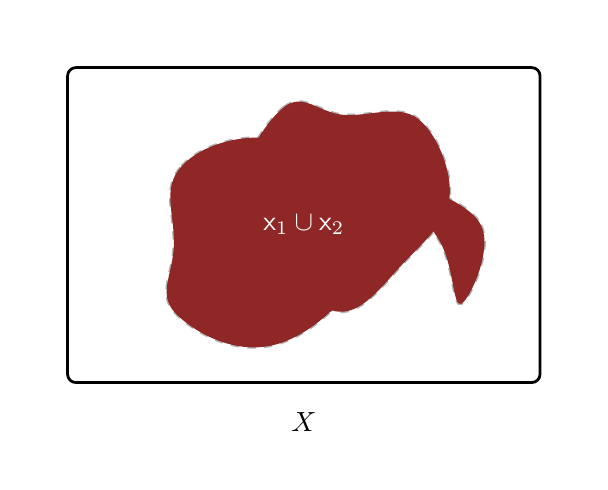
\begin{tikzpicture}[scale=1.0]
  
  \draw[white] (-3.5, -3) rectangle (3.5, 2.5);

  \draw[rounded corners=3, color=black, line width=1] (-3, -2) rectangle (3, 2);
  \node at (0, -2.5) { $X$ };
    
  \draw[gray70, dashed, line width=1] plot [smooth cycle, tension=0.75] coordinates { 
    (-1.65, -0.25) (-1.55, 0.75) (-0.4, 1.1) (0.3, 0.5) 
    (0.85, -0.35) (-0.3, -1.5) (-1.6, -1.15) } -- cycle;
  
  \draw[gray70, dashed, line width=1] plot [smooth cycle, tension=0.65] coordinates { 
    (-0.85, 0.35) (-0.25, 1.5) (0.5, 1.4) (1.45, 1.35) 
    (1.85, 0.35) (1.25, -0.5) (0.5, -1.1) (-0.25, -0.6) } -- cycle;
  
  \draw[gray70, dashed, line width=1] plot [smooth cycle, tension=0.75] coordinates { 
    (1.25, 0.5) (2.25, 0) (2, -1) (1.75, -0.25)} -- cycle; 
  
  \fill[dark] plot [smooth cycle, tension=0.75] coordinates { 
    (-1.65, -0.25) (-1.55, 0.75) (-0.4, 1.1) (0.3, 0.5) 
    (0.85, -0.35) (-0.3, -1.5) (-1.6, -1.15) } -- cycle;
  
  \fill[dark] plot [smooth cycle, tension=0.65] coordinates { 
    (-0.85, 0.35) (-0.25, 1.5) (0.5, 1.4) (1.45, 1.35) 
    (1.85, 0.35) (1.25, -0.5) (0.5, -1.1) (-0.25, -0.6) } -- cycle;
    
  \fill[dark] plot [smooth cycle, tension=0.75] coordinates { 
    (1.25, 0.5) (2.25, 0) (2, -1) (1.75, -0.25)} -- cycle; 
  
  \node[white] at (0, 0) { $\mathsf{x}_{1} \cup \mathsf{x}_{2}$ };

  
\end{tikzpicture}

\end{document}  